\documentclass[12pt]{article}
\usepackage{fullpage,enumitem,amsmath,amssymb,graphicx}
\usepackage{listings}
\usepackage{tikz}
\usepackage{hyperref}
\usepackage{bbm}

\newcommand{\vect}[1]{\boldsymbol{#1}}

\begin{document}

\begin{center}
{\Large CS 228 Winter 2018 Homework 4}

\begin{tabular}{rl}
SUNet ID: & 05794739 \\
Name: & Luis Perez \\
Collaborators: & \\
Late Days: & 0
\end{tabular}
\end{center}

By turning in this assignment, I agree by the Stanford honor code and declare
that all of this is my own work.

\section*{Problem 1}

\begin{enumerate}[label=(\alph*)]
  \item We compute the acceptable probability for each MH step. We first introduce some notation to make things easier. Let $C$ a random vector consisting of $C_1, \cdots, C_K$ (ie, it corresponds to one particular assignment of correspondance variables) such that $Val(C) = perm(\{1,\cdots, K\})$ where $perm$ returns all possible permutations of the input set. Let $v$ be a random vector corresponding to $v_1, \cdots, v_k$ such that $Val(v) = \{a_1, \cdots, a_L\}^K$.

  We will use MH to approximate sampling from the distribution $P(C = c\mid v = a)$. Our proposal distribution will be $Q(C = c' \mid C = c, v = a)$ which randomly selects two indexes of $c$ (uniformly) and swaps ther values.

  With the previous definition, have
  \begin{align*}
  	A(x' \mid x) &= A(c' \mid c) \\
  	&= \min \left\{1, \frac{P(C = c' \mid v = a)Q(C = c \mid C = c', v = a)}{P(C = c \mid v = a)Q(C = c' \mid C = c, v = a)} \right\}
  \end{align*}

  We first note that $Q(C = c' \mid C = c, v = a) = Q(C = c \mid C = c', v = a)$. The reasoning is obvious, since the probability of going from assignment $c' \to c$ is exactly equal to the probability of going from $c \to c'$ since we would need to swap the same two indexes $i$ and $j$. We can thefore simplify the term in the min to:
  \begin{align*}
  	\frac{P(C = c' \mid v = a)}{P(C = c \mid v = a)} &= \frac{\frac{P(v= a \mid C = c')P(C = c')}{P(v = a)}}{\frac{P(v= a \mid C = c)P(C = c)}{P(v = a)}} \tag{Bayes Rule} \\
  	&= \frac{P(v = a \mid C = c')P(C = c')}{P(v = a \mid C = c)P(C = c)} \tag{Normalization Cancels}\\
  	&= \frac{P(v = a \mid C = c')}{P(v = a \mid C = c)}\tag{We assume uniform prior over all possible assignments, so $P(C = c') = P(C = c)$} \\
  	&= \frac{P(v_1 = a_1, \cdots, v_K = a_K \mid C_1 = c'_1, \cdots, C_K = c'_K)}{P(v_1 = a_1, \cdots, v_K = a_K \mid C_1 = c_1, \cdots, C_K = c_K)} \\
  	&= \frac{\prod_{i=1}^K P_i(v_i = a_i \mid C_i = c'_i )}{\prod_{i=1}^K P_i(v_i = a_i \mid C_i = c_i )} \tag{We assume that $\forall i,j \in [1,\cdots, K], v_i \perp v_j \mid C_1, \cdots, C_K$ and $v_i \perp C_j \mid C_i$} \\
  	&= \frac{P_i(v_i = a_i \mid C_i = c_j)P_j(v_j = a_j \mid C_j = c_i)}{P_i(v_i = a_i \mid C_i = c_i)P_j(v_j = a_j \mid C_j = c_j)} \tag{Since we know that $c'$ and $c$ differ only by the swapped $i,j$ assigments}
  \end{align*}
  We note that it is reasonable to assume $\forall i,j \in [1,\cdots, K], v_i \perp v_j \mid C_1, \cdots, C_K$ since given all of the correspondances for the observations, they are independent. Furthermore, it makes sense to $v_i \perp C_j \mid C_i$, since knowing the object to which measurement $v_i$ corresponds, the measurement is then independent from the other assignments. From the above, we arrive at the final equation for the acceptance probability of assignments $c'$ where we picked variables $C_i$ and $C_j$ to be swapped:
  \begin{align*}
  A(c' \mid c) &= \min\left\{1, \frac{P_i(v_i = a_i \mid C_i = c_j)P_j(v_j = a_j \mid C_j = c_i)}{P_i(v_i = a_i \mid C_i = c_i)P_j(v_j = a_j \mid C_j = c_j)} \right\}
  \end{align*}

  \item Once we have run the MH sampler for a long time (the burn-in period), when we collect the $M$ samples $C_1[m], \cdots, C_k[m]$, we expect these to be samples from the true distribution $P(C = c \mid v = a)$. Therefore, to estimate the marginal $P(C_i = c_i \mid v = a)$, we can directly use a Monte Carlo estimate.
  \begin{align*}
  	P(C_i = c_i \mid v = a) &= \sum_{c_{-i}} P(C_i = c_i, C_{i-1} = c_{-i}) \\
  	&= \sum_{c_i} \mathbbm{1}[C_i = c_i]P(C_1 = c_1, \cdots, C_K = c_k) \\
  	&= E_{P(C \mid v)}[g(c)] \tag{Where $g(c) = \mathbbm{1}[C_i = c_i]$}\\
  	&\approxeq \frac{1}{M} \sum_{m = 1}^M g(C_1[m], \cdots, C_K[m]) \\
  	&= \frac{\#\text{ samples with }C_i = c_i}{M}
  \end{align*}
  \item The naive version of Gibbs sampling would not directly work. Gibbs sampling where we sample one variable by holding all others fixed. It is just a special case of MH where the proposal distribution would look like: 
  $$
  	Q(C_i = c_i' \mid C_{i} = c_i, C_{-i} = c_{-i}, v= a) = P(C_i = c_i' \mid C_{-i} = c_{-i} ,v=a)
  $$
  However, due to the mutext constraints on the $C_i$ variables, the above would simply give us:
  $$
  P(C_i = x \mid C_{-i} = c_{-i} ,v=a) = \begin{cases} 
      1 & x = c_i \\
      0 & x \neq c_i 
   \end{cases}
	$$
	which means we will never move to a different configuration. Basically, leaving all $C_i$ fixed but one necessarily forces that $C_i$ to be the only unassigned value. We could modify Gibbs sampling so that we leave all $C_i$ fixed except $2$, but this is not the typical proposal distribution people have in mind when they discuss Gibbs sampling.
\end{enumerate}

\section*{Problem 2}

\begin{enumerate}[label=(\alph*)]
  \item We write down the full objective function in terms of $f_i$ and $\theta_i$. This is simply an exercise in symbol manipulation.
  \begin{align*}
  	g(\vect{\theta}; \mathcal{D}) &= (1-\alpha)\ell_{\vect{Y}\mid \vect{X}}(\vect{\theta}; \mathcal{D}) + \alpha\ell_{\vect{X}\mid\vect{Y}}(\vect{\theta}; \mathcal{D}) \\
  	&= (1- \alpha)\log \prod_{m=1}^M P_{\theta}(\vect{x}^m \mid \vect{y}^m) + \alpha \log \prod_{m=1}^M P_{\theta}(\vect{y}^m \mid \vect{x}^m) \\
  	&= (1- \alpha)\sum_{m=1}^M \log P_{\theta}(\vect{x}^m \mid \vect{y}^m) + \alpha \sum_{m=1}^M \log P_{\theta}(\vect{y}^m \mid \vect{x}^m)
  \end{align*}
  Let us define the following, to simplify notation:
  \begin{align*}
  	Z_{\vect{y}^m} &= \sum_{\vect{x}} \exp\left(\sum_{i =1}^n \theta_i f_i(\vect{x}_i, \vect{y}^m_i)\right) \\
  	Z_{\vect{x}^m} &= \sum_{\vect{y}} \exp\left(\sum_{i =1}^n \theta_i f_i(\vect{x^m}_i, \vect{y}_i)\right) \\
  	Z &= \sum_{\vect{x}, \vect{y}} \exp\left(\sum_{i=1}^n \theta_i f_i(\vect{x}_i, \vect{y}_i)\right)
  \end{align*}
  Now, let us focus on one part of the above (the other can be similarly simplified). 
  \begin{align*}
  	\log P_{\theta}(\vect{x}^m \mid \vect{y}^m) &= \log P_{\theta}(\vect{x}^m, \vect{y}^m) - \log P_{\theta}(\vect{y}^m) \tag{Bayes Rule} \\
  	&= \log P_{\theta}(\vect{x}^m, \vect{y}^m) - \log \left(\sum_{\vect{x}} P_{\theta}(\vect{x}, \vect{y}^m)\right)\\
  	&= \log P_{\theta}(\vect{x}^m, \vect{y}^m) - \log Z_{\vect{y}^m} \\
  	&= \log \exp(\sum_{i=1}^n \theta_i f_i(\vect{x}^m_i, \vect{y}^m_i)) - \log Z - \log Z_{\vect{y}^m} \\
  	&= \sum_{i=1}^n \theta_i f_i (\vect{x}_i^m, \vect{y}_i^m) - \log Z - \log Z_{\vect{y}^m}
  \end{align*}
  Similarly we have:
  $$
		\log P_{\theta}(\vect{y}^m \mid \vect{x}^m) = \sum_{i=1}^n \theta_i f_i (\vect{x}_i^m, \vect{y}_i^m) - \log Z - \log Z_{\vect{x}^m}
  $$
  Plugging into our original equation and subtituting back our definitions to obtain the fully expanded form:
  \begin{align*}
  	g(\vect{\theta}; \mathcal{D}) &= (1- \alpha)\sum_{m=1}^M \log P_{\theta}(\vect{x}^m \mid \vect{y}^m)  + \alpha \sum_{m=1}^M  \log P_{\theta}(\vect{y}^m \mid \vect{x}^m) \\
  	&= (1- \alpha)\sum_{m=1}^M \left[\sum_{i=1}^n \theta_i f_i (\vect{x}_i^m, \vect{y}_i^m) - \log Z - \log Z_{\vect{y}^m}\right]  \\
  	&+ \alpha \sum_{m=1}^M \left[\sum_{i=1}^n \theta_i f_i (\vect{x}_i^m, \vect{y}_i^m) - \log Z - \log Z_{\vect{x}^m}\right] \\
  	&= -M\log Z  + \sum_{m=1}^M \left[\sum_{i=1}^n \theta_i f_i(\vect{x}_i^m, \vect{y}_i^m) - (1-\alpha) \log Z_{\vect{y}^m} - \alpha \log Z_{\vect{x}^m} \right] \\
  	&= -M \log \left(\sum_{\vect{x}, \vect{y}} \exp\left(\sum_{i=1}^n \theta_i f_i(\vect{x}_i, \vect{y}_y)\right) \right) \\
  	&+ \sum_{m=1}^M \sum_{i=1}^n \theta_i f_i(\vect{x}_i^m, \vect{y}_i^m) \\
  	&- (1-\alpha) \sum_{m=1}^M \log \left(\sum_{\vect{x}} \exp\left(\sum_{i =1}^n \theta_i f_i(\vect{x}_i, \vect{y^m}_i)\right)\right) \\
  	&- \alpha \sum_{m=1}^M \log \left(\sum_{\vect{y}} \exp\left(\sum_{i =1}^n \theta_i f_i(\vect{x^m}_i, \vect{y}_i)\right) \right)
  \end{align*}
  \item We are interested in computing the derivative $\frac{\partial}{\partial \theta_i}$. Again, this is just an exercise in symbol manipulation. We first note the following relations:
  \begin{align*}
  	\frac{\partial \log Z_{\vect{y}^m}}{\partial \theta_i} &= \frac{1}{Z_{\vect{y}^m}} \sum_{\vect{x}} \frac{\partial}{\partial \theta_i} \exp\left(\sum_{i =1}^n \theta_i f_i(\vect{x}_i, \vect{y}^m_i)\right) \\
  	&= \frac{1}{Z_{\vect{y}^m}} \sum_{\vect{x}} f_i(\vect{x}_i, \vect{y}_i^m) \exp\left(\sum_{i =1}^n \theta_i f_i(\vect{x}_i, \vect{y}^m_i)\right)  \\
  	&= Z \sum_{\vect{x}} f_i(\vect{x}_i, \vect{y}_i^m) \frac{\exp\left(\sum_{i =1}^n \theta_i f_i(\vect{x}_i, \vect{y}^m_i)\right) }{Z Z_{\vect{y}^m}} \\
  	&= ZE_{P_{\vect{\theta}}(\vect{X} \mid \vect{Y} = \vect{y}^{m})}[f_i(\vect{x}_i, \vect{y}_i^m)]
  \end{align*}
  Similarly, we have:
  $$
  	\frac{\partial\log Z_{\vect{x}^m}}{\partial \theta_i}  = ZE_{P_{\vect{\theta}}(\vect{Y} \mid \vect{X} = \vect{x}^{m})}[f_i(\vect{x}_i^m, \vect{y}_i)]
  $$
  And lastly, we have:
  \begin{align*}
  	\frac{\partial \log Z}{\partial \theta_i} &= \frac{1}{Z} \sum_{\vect{x}, \vect{y}} \frac{\partial}{\partial \theta_i} \exp\left(\sum_{i =1}^n \theta_i f_i(\vect{x}_i, \vect{y}_i)\right) \\
  	&= \frac{1}{Z} \sum_{\vect{x}, \vect{y}} f_i(\vect{x}_i, \vect{y}_i) \exp\left(\sum_{i =1}^n \theta_i f_i(\vect{x}_i, \vect{y}_i)\right)  \\
  	&= \sum_{\vect{x}, \vect{y}} f_i(\vect{x}_i, \vect{y}_i) \frac{\exp\left(\sum_{i =1}^n \theta_i f_i(\vect{x}_i, \vect{y}_i)\right) }{Z} \\
  	&= E_{P_{\vect{\theta}}(\vect{X}, \vect{Y})}[f_i(\vect{x}_i, \vect{y}_i)]
  \end{align*}
  Putting the above together, we have:
  \begin{align*}
  	\frac{\partial }{\partial \theta_i}g(\vect{\theta};D) &= -M\frac{\partial }{\partial \theta_i} \log Z + \sum_{m=1}^M\left[ \sum_{i=1}^n \frac{\partial }{\partial \theta_i} \theta_i f_i(\vect{x}_i^m, \vect{y}_i^m) - (1-\alpha)\frac{\partial }{\partial \theta_i} \log Z_{\vect{y}^m} - \alpha \frac{\partial }{\partial \theta_i}\log Z_{\vect{x}^m} \right] \\
  	&= \sum_{i=1}^M f_i(\vect{x}_i^m, \vect{y}_i^m) \\
  	&- ME_{P_{\vect{\theta}}(\vect{X}, \vect{Y})}[f_i(\vect{x}_i, \vect{y}_i)] \\
  	&- Z(1-\alpha)\sum_{m=1}^M E_{P_{\vect{\theta}}(\vect{X} \mid \vect{Y} = \vect{y}^{m})}[f_i(\vect{x}_i, \vect{y}_i^m)] \\
  	&- Z\alpha\sum_{m=1}^M E_{P_{\vect{\theta}}(\vect{Y} \mid \vect{X} = \vect{x}^{m})}[f_i(\vect{x}_i^m, \vect{y}_i)] \\
  	&= M\hat{E}[f_i(\vect{x}_i^m, \vect{y}_i^m)] \tag{Sample Mean} \\
  	&- ME_{P_{\vect{\theta}}(\vect{X}, \vect{Y})}[f_i(\vect{x}_i, \vect{y}_i)] \tag{True Mean}\\
  	&- Z(1-\alpha)\sum_{m=1}^M E_{P_{\vect{\theta}}(\vect{X} \mid \vect{Y} = \vect{y}^{m})}[f_i(\vect{x}_i, \vect{y}_i^m)] \tag{Conditional Expectation $X \mid Y$}\\
  	&- Z\alpha\sum_{m=1}^M E_{P_{\vect{\theta}}(\vect{Y} \mid \vect{X} = \vect{x}^{m})}[f_i(\vect{x}_i^m, \vect{y}_i)] \tag{Condtional Expectation $Y \mid X$}
  \end{align*}
\end{enumerate}


\section*{Problem 3}

\begin{enumerate}[label=(\alph*)]
	\item We show that the EM algorithm converges in one iteration and we give a closed form expression for the parameter values at this point. In other words, we give a closed form expressions for $\theta_c^1$ and $\theta^1_{x_i} \mid c$. We initialize the algorithm by setting:
	$$
		\theta_c^0 = \frac{1}{|Val(C)|}, \theta_{x_i \mid c}^0 = \frac{1}{|Val(X_i|}
	$$
	In our case, the missing data is $c$, therefore, we begin with the $E$ step where we ``hallucinate'' the possible values of $c$ given each of our training examples. For each example $\vect{x}[m]$, we compute:
	\begin{align*}
		Q^1(C = c \mid X = x[m]) &= P(C = c \mid X = x[m], \theta^0_c, \theta^0_{x_1 \mid c}, \cdots, \theta^0_{x_n \mid c}) \\
		&= \frac{P(X = x[m] \mid C = c, \theta^0_{x_1}, \cdots,\theta^0_{x_n})P(C \mid \theta^0_c)}{\sum_{c} P(X = x[m] \mid C = c, \theta^0_{x_1}, \cdots, \theta^0_{x_n})P(C \mid \theta^0_c)} \tag{Bayes Rule and Conditional Independence} \\
		&= \frac{\prod_i P(X_i = x_i[m] \mid C = c, \theta^0_{x_i})P(C \mid \theta_c^0)}{\sum_c \prod_i P(X_i = x_i[m] \mid C = c, \theta^0_{x_i})P(C \mid \theta_c^0)} \\
		&= \frac{\prod_i \frac{1}{|Val(X_i)|} \frac{1}{|Val(C)|}}{\sum_c \prod_i \frac{1}{|Val(X_i)|} \frac{1}{|Val(C)|}} \\
		&= \frac{\frac{1}{|Val(C)|}\prod_i \frac{1}{|Val(X_i)|}}{\prod_i \frac{1}{|Val(X_i)|} \sum_c \frac{1}{|Val(C)|}} \\
		&= \frac{\frac{1}{|Val(C)|}}{\sum_c \frac{1}{|Val(C)|}} \\
		&= \frac{1}{|Val(C)|}
	\end{align*}
	The next step is simply to maximize the expectation of the log likelihood over these ``hallucinated'' values for each data point. That is to say, we have the objective function:
	\begin{align*}
		f(\theta) &= \sum_{m=1}^M E_{Q^1(C = c[m] \mid X = x[m])}[\log p(x[m], c[m]; \theta)] \\
		&= \sum_{m=1}^M E_{c[m] \sim Uniform(\frac{1}{|Val(C)|})}[\log p(x[m], c[m]; \theta)] 
	\end{align*}
	And we wish to compute:
	$$
		\theta_1 = \arg\max_{\theta} f(\theta)
	$$
	subject to the constraints $\sum_{c} \theta_c = 1$ and $\forall c, \sum_{x_i} \theta_{x_i \mid c} = 1$.
	From lecture, we know that the above is maximized by the parameters:
	\begin{align*}
		\theta_c &= 
		\frac{1}{M}\sum_{m=1}^M \sum_{\hat{c}[m]} \mathbbm{1}[\hat{c[m]} = c]
		\\
		\theta_{x_i \mid c} &= \frac{\sum_{m=1}^M \sum_{\hat{c}[m]} \mathbbm{1}[c[m] = x, x[m]_i = x_i] }{\sum_{m=1}^M \sum_{\hat{c}[m]} \mathbbm{1}[c[m] = x]}
	\end{align*}
	With the above, we have now a closed form solution.
\end{enumerate}

\section*{Problem 4}

\begin{enumerate}[label=(\alph*)]
\item We derive the expression for the condtional probability of the pixel $(i,j)$ is back given its Markov Blanket. In other words, we compute $p(y_{ij} = 1 \mid y_{M_(i,j)})$ where $y_{M(i,j)}$ denotes the Markov blanket. We also introduce the notation $y_{\bar{M}(i,j)}$ to mean all variables not in the Markov blanket and not $y_{ij}$, Note that we have $y_{M(i,j)} = \{x_{ij}, y_{N(i,j)}\}$ where $y_{N(i,j)}$ denotes the neighboring pixels of $y_{i,j}$. Furthermore, let $E \setminus (i,j)$ denote the set of all edges excluding edges where $(i,j)$ is an endpoint. Furthermore, for $((i,j), (i',j')) = e \in E$, denote $e_1 = (i,j)$ and $e_2 = (i',j')$. Wih the above notation out of the way, we have:
\begin{align*}
&p(y_{ij} = 1 \mid y_{M(i,j)}) \\
&= p(y_{ij} = 1 \mid x_{ij}, y_{N(i,j)}) \\
&= \frac{\sum_{\bar{M}(i,j)} p(y_{ij} = 1, x_{ij}, y_{N(i,j)}, y_{\bar{M}(i,j)}) }{\sum_{y_{ij}}\sum_{\bar{M}(i,j)} p(y_{ij}, x_{ij}, y_{N(i,j)}, y_{\bar{M}(i,j)}} \\
&= \frac{\frac{1}{Z} \exp[\eta x_{ij}] \prod_{y_{i'j'} \in y_{N(i,j)}} \exp[\beta y_{i'j'}] \sum_{\bar{M}(i,j)}\prod_{n \neq i}\prod_{m \neq j}\exp[\eta y_{nm}x_{nm}] \prod_{e \in E \setminus (i,j)} \exp[\beta y_{e_1}y_{e_2}] }{\frac{1}{Z} \sum_{y_{ij}} \exp[\eta y_{ij}x_{ij}] \prod_{y_{i'j'} \in y_{N(i,j)}} \exp[\beta y_{ij}y_{i'j'}] \sum_{\bar{M}(i,j)}\prod_{n \neq i}\prod_{m \neq j}\exp[\eta y_{nm}x_{nm}] \prod_{e \in E \setminus (i,j)} \exp[\beta y_{e_1}y_{e_2}]} \\
&= \frac{\exp [\eta x_{ij} + \beta \sum_{y_{i'j'} \in y_{N(i,j)}} y_{i'j'}]}{\exp [\eta x_{ij} + \beta \sum_{y_{i'j'} \in y_{N(i,j)}} y_{i'j'}] + \exp [-\eta x_{ij} - \beta \sum_{y_{i'j'} \in y_{N(i,j)}} y_{i'j'}]} \\
&= \frac{\exp (2[\eta x_{ij} + \beta \sum_{y_{i'j'} \in y_{N(i,j)}} y_{i'j'}])}{\exp (2[\eta x_{ij} + \beta \sum_{y_{i'j'} \in y_{N(i,j)}} y_{i'j'}]) + 1} \\
&= \sigma(2\eta x_{ij} + 2\beta\sum_{y_{i'j'} \in y_{N(i,j)}} y_{i'j'})
\end{align*}
Where we define $\sigma(x) = \frac{e^x}{1 + e^x}$.
Being explicity, we have the following two results. For $i \not\in \{1,N\}, j \not\in \{1,M\}$:
\begin{align*}
	p(y_{ij} = 1 \mid y_{M(i,j)}) &= p(y_{ij} = 1 \mid y_{i-1, j}, y_{i, j-1}, y_{i+1, j}, y_{i, j + 1}, x_{ij}) \\
	&= \sigma(2\beta[y_{i-1,j} + y_{i, j-1} + y_{i+1,j}+y_{i,j+1}] + 2\eta x_{ij})
\end{align*}
and for $i \in \{1,N\}, j \in \{1, M\}$:
\begin{align*}
	p(y_{11} = 1 \mid y_{M(1,1)}) &= p(y_{11} = 1 \mid y_{21}, y_{12}, x_{11}) \\
	&= \sigma(2\beta[y_{21}+y_{12}] + 2\eta x_{11}) \\
	p(y_{NM} = 1 \mid y_{M(1,1)}) &= p(y_{NM} = 1 \mid y_{N-1, M}, y_{N, M-1}, x_{NM}) \\
	&= \sigma(2\beta[y_{N-1, M}+y_{N, M-1}] + 2\eta x_{NM}) \\
	p(y_{1M} = 1 \mid y_{M(1,M)}) &= p(y_{1M} = 1 \mid y_{1, M-1}, y_{2M}, x_{1M}) \\
	&= \sigma(2\beta[y_{1, M-1} + y_{2M}] + 2\eta x_{1M}) \\
	p(y_{N1} = 1 \mid y_{M(N,1)}) &= p(y_{N1} = 1 \mid y_{N-1, 1}, y_{N2}, x_{N1}) \\
	&= \sigma(2\beta[y_{N-1,1} +y_{N2}] + 2\eta x_{N1}) \\
	p(y_{1j} = 1 \mid y_{M(1,j)}) &= p(y_{1j} = 1 \mid y_{2j}, y_{1,j+1}, y_{1, j-1} x_{1j}) \\
	&= \sigma(2\beta[y_{2j}+y_{1,j+1} + y_{1, j-1}] + 2\eta x_{1j}) \tag{$j \neq 1,M$} \\
	p(y_{i1} = 1 \mid y_{M(i,1)}) &= p(y_{i1} = 1 \mid y_{i-1, 1}, y_{i+1, 1}, y_{i, 2}, x_{i1}) \\
	&= \sigma(2\beta[y_{i-1, 1}+y_{i+1, 1} + y_{i,2}] + 2\eta x_{i1} \tag{$i \neq 1, N$}) \\
	p(y_{iM} = 1 \mid y_{M(i,M)}) &= p(y_{iM} = 1 \mid y_{i, M-1}, y_{i+1, M}, y_{i-1, M}, x_{iM}) \\
	&= \sigma(2\beta[y_{i, M-1} + y_{i+1, M} + y_{i-1, M}] + 2\eta x_{iM}) \tag{$i \neq 1, N$} \\
	p(y_{Nj} = 1 \mid y_{M(N,j)}) &= p(y_{Nj} = 1 \mid y_{N-1, j}, y_{N, j+1}, y_{N, j-1}, x_{Nj}) \\
	&= \sigma(2\beta[y_{N-1,j} +y_{N, j+1} + y_{N, j - 1}] + 2\eta x_{Nj}) \tag{$j \neq 1, M$}
\end{align*}

\item We outline the Gibbs sampling algorithm in pseudo-code that samples from $p(\vect{y} \mid \vect{x})$.
	\begin{itemize}
		\item Set $\vect{x}$ to the observed values. 
		\item Initialize $\vect{y}$ to be equal to $\vect{x}$ (in theory, we could use any initialization, but it seems ``sensible'' to start with a ``good'' guess -- in this case, the corrupted image should be ``close'' to the real image, so it's a decent guess to start).
		\item For $B$ steps:
			\begin{itemize}
				\item For $i \gets 1$ to $i = N$
				 	\begin{itemize}
				 		\item For $j \gets 1$ to $i = M$
				 			\begin{itemize}
				 				\item Compute $2\eta \vect{x}_{ij} + 2\beta\sum_{\vect{y}_{i'j'} \in \vect{y}_{N(i,j)}} \vect{y}_{i'j'}$. This can be done by summing the values of each neighbor of pixel $(i,j)$ (according to $\vect{y}$), doubling the result and multiplying by $\beta$, and then adding the value of $2\eta x_{ij}$. Note that each pixel has at most four neighbors, so this calculation takes a constant amount of work.
				 				\item Run the result from above through the $\sigma$ function -- again, this takes constant time. Let this result be $p_{ij}$.
				 				\item Generate a random sample $r \sim Uniform(0,1)$.
				 				\item If $r \leq p_{ij}$, update $\vect{y}_{ij} = 1$. Otherwise, set $\vect{y}_{ij} = -1$. Note that we do a mutation of $\vect{y}$, so this value will persist.
				 			\end{itemize}
				 	\end{itemize}
			\end{itemize}
		\item Repeat for $s \geq 1$ to $S$:
			\begin{itemize}
				\item Allocate space for $\vect{y[s]}$ (ie, a vector of size $NxM$).
				\item For $i \gets 1$ to $i = N$
				 	\begin{itemize}
				 		\item For $j \gets 1$ to $i = M$
				 			\begin{itemize}
				 				\item Repeat the corresponding first three steps from above to generate $r, p_{ij}$. Note that we still use $\vect{x}$ and $\vect{y}$.
				 				\item If $r \leq p_{ij}$, set $\vect{y[s]}_{ij} = 1$. Otherwise, set $\vect{y[s]}_{ij} = -1$. We do NOT mutate $\vect{y}$ (though, technically, since we're assuming we've converged, mutating it should not make a difference)
				 			\end{itemize}
				 	\end{itemize}
			\end{itemize}
		\item Return the $S$ samples $\vect{y[s]}$ generated above.
	\end{itemize}

	We note that by construction, the stationary distribution of our Markov Process above is $p(\vect{y} \mid \vect{x})$. Therefore, it is straightforward to ensure that the above process will actually generate samples from $p(\vect{y} \mid \vect{x})$ for large enough values of $B$. We simply need to ensure that the chain is ergodic to guarantee convergence.

	We note that to ensure irreducibility, we simply need to guarantee that we can potentially move to any state of the vector $\vect{y}$. We note that this immediately follows from the fact that $p(y_{ij} = 1 \mid y_{M(i,j)}) = \sigma(...)$, since this guarantees that $0 < p(y_{ij} = 1 \mid y_{M(i,j)}) < 1$. Therefore it is possible to transition from any state $\vect{y}$ to any other state $\vect{y}'$.

	To ensure the chain is aperiodic, we note that for any state $\vect{y}$, there is always a non-zero probability that we will change non of its values (for similar reasons outlined above), and therefore the chain has a period of $1$ (aperiodic).

	With the above, we know the chain is ergodic, and therefore by construction, we know that the equilibrium distribution is in fact the posterior distributions $p(\vect{y} \mid \vect{x})$.

\item We implement the above algorutnm and apply it to the image with $20\%$, using values of $\eta = 1, \beta = 1, B = 100, S = 1000$. On each iteration, we compute $E(\vect{y}, \vect{x})$. We run the algorithm with three distinct initializations of $y_ij$. (1) same as $x_{ij}$, (2) negative of $x_{ij}$ and (3) random. We plot these values in Figure \ref{fig:log_energies}.

\begin{figure}[h!]
\centering
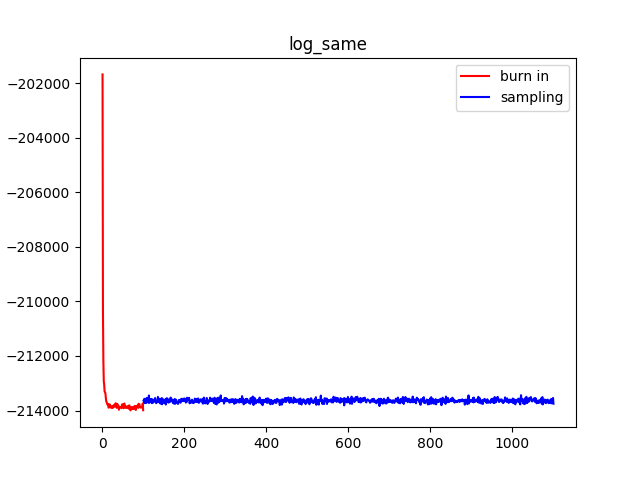
\includegraphics[scale=0.5]{programming/log_same.png}
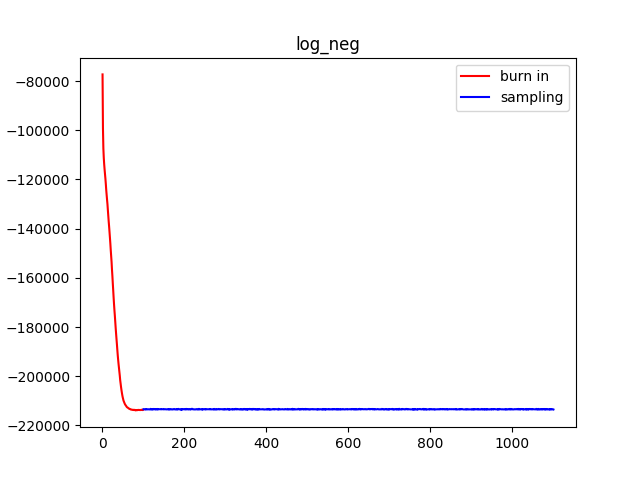
\includegraphics[scale=0.5]{programming/log_neg.png}
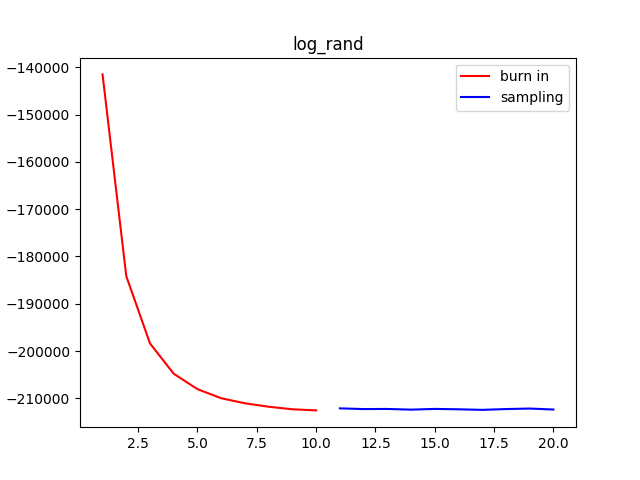
\includegraphics[scale=0.5]{programming/log_rand.png}
\caption{t}
\label{fig:log_energies}
\end{figure}

From the figure, we can tell that all three initializations appear to be converging to the same energy region in the posterior (some state with $E(\vect{x}, \vect{y}) \approxeq -214000$.
\end{enumerate}
\end{document}
